\subsection{Pitch Generation}\label{subsec:Pitch_Generation}

Die Hauptaufgabe der Komponente Pitch Generation ist es das Audiosignal aus dem Rechtecksignal der Tonhöhenantenne (Pitch Antenna) zu generieren. Pitch Generation nimmt zudem eine Frequenzmessung des Audiosignals vor um diverse Funktionalitäten zu gewährleisten. In Abbildung \ref{img:Blockschaltbild_pitch} ist der Grobe aufbau der Komponente aufgezeigt. Die genaue Erklärung zu den einzelnen Komponenten ist in den folgenden Abschnitten zu finden.


\begin{figure}[h!]
	\centering
	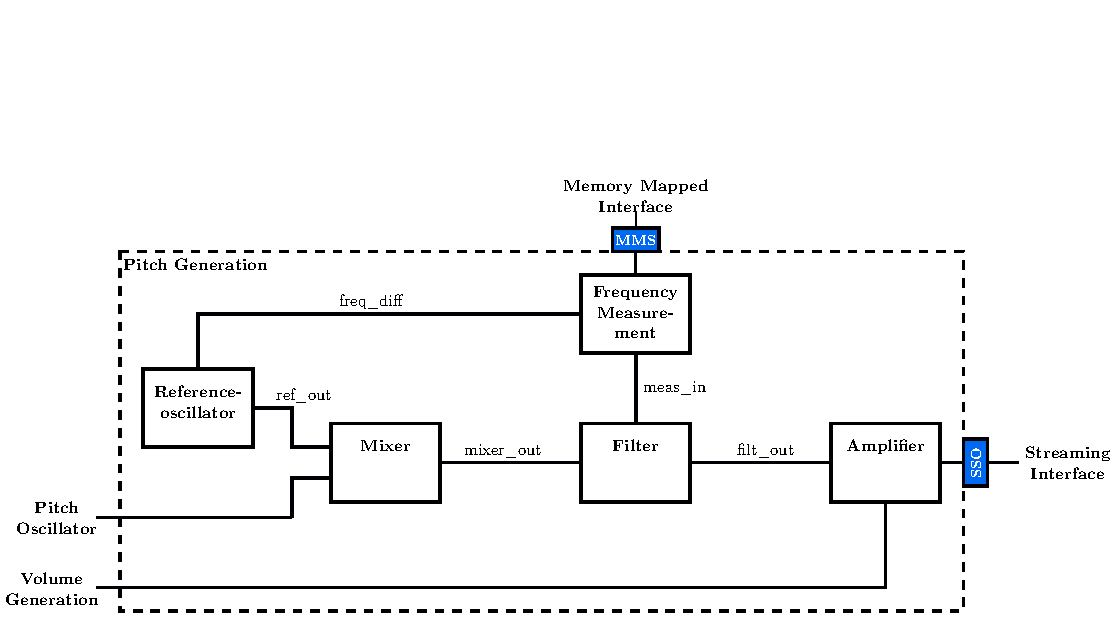
\includegraphics[width=1\textwidth]{Blockschaltbild_pitch.pdf}
	\caption{Blockschaltbild der Custom IP Pitch Generation} 
	\label{img:Blockschaltbild_pitch}
\end{figure}  



\paragraph{Referenzoszillator}\mbox{}\\

Der Referenzoszillator ist wie in Kapitel ... \todo{Referenz auf Grundlagen digitales Theremin} dafür zuständig ein Sinussignal mit einer Frequenz nahe der des Antennenoszillator zu generieren. Er generiert diesen wie schon erwähnt mithilfe des Cordic Algorithmus. Er ist aufgeteilt in zwei Komponenten: der Cordic Processor und der Cordic Controller. Wie diese beiden Komponenten miteinander verbunden sind ist in Abbildung \ref{img:Referenceoscillator} ersichtlich. Beide Komponenten stammen aus dem Projekt 5. Änderungen, welche im Projekt 6 stattfanden, sind entsprechend gekennzeichnet. \\

\begin{figure}[h!]
	\centering
	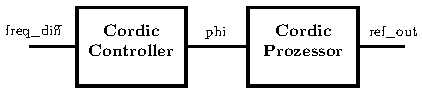
\includegraphics[width=0.53\textwidth]{Referenceoscillator.pdf}
	\caption{Aufbau des Referenzoszillators} 
	\label{img:Referenceoscillator}
\end{figure}  

Der Cordic Processor ist die eigentliche Implementierung des Cordic Algorithmus wie er in Kapitel ... \todo{Referenz auf Cordic Kapitel einfügen} beschrieben wurde. Er muss jedoch für den Einsatz im FPGA leicht angepasst werden. \\
Die Berechnung der Werte für \(\arctan{2^{-i}}\) konnte vorgängig gemacht werden und ist in eine Lookup Table gespeichert. Dies spart Ressourcen für diese komplizierte Berechnung ein. Wir haben uns entschieden den Algorithmus in einer Pipeline zu implementieren. Dies führt einerseits zu einer höheren maximalen Clockfrequenz, andererseits aber auch zu einer grösseren Signallatenz. Dies ist jedoch nicht problematisch für die gewählte Anwendung, da die Latenz im Nanosekundenbereich ist und später nicht hörbar auffällt. Zuletzt ist eine Multiplikation mit \(2^{-i}\) ganz einfach durch eine Verschiebung um \(i\) Bits nach rechts ersetzbar. Dies spart wiederum Ressourcen ein.\\
Das berechnete Resultat ist als signed Zahl definiert um die Berechnung von negativen Zahlen zu ermöglichen. Sie sind im fixed-point Format und haben \SI{16}{Bit} Länge. Dabei sind von den \SI{16}{Bit} \SI{1}{Bit} Vorzeichen und \SI{15}{Bit} Nachkommastellen. Dies entspricht einem Zahlenbereich von -1 bis 0.999969.

Für die Berechnung der Sinuswerte muss ein Winkelwert berechnet werden, der mit der Zeit so ändert, dass sich am Ausgang des Cordic Processor ein Sinus mit der gewünschten Frequenz ergibt. Für diese Aufgabe ist der Cordic Controller zuständig. Bei mit der Zeit linear ansteigendem Winkelwert ergibt sich am Ausgang die gewünschte Sinusform. Wichtig ist jedoch, dass der Cordic Algorithmus nur für Winkelwerte zwischen  \(-\pi/2\) und \(\pi/2\) der anders für Werte im ersten und zweiten Quadranten konvergiert. Die Lösung für dieses Problem ist in Abbildung \ref{img:Cordic_phi} ersichtlich. 
Als erstes wird der Sägezahn Winkel berechnet. Für den linearen Anstieg des Winkels zählt der Cordic Controller einen Zähler mit einer bestimmten Schrittweite jeden Clockzyklus hoch. Der wrap-around des Zählers ist dabei sogar erwünscht um den Sprung zwischen dem II und III Quadranten zu erzielen. Der Schrittwert ergibt sich wie folgt:

\begin{equation}
step = \frac{2^{n+1}f_{sig}}{f_{clk}}
\label{equ:cordic_3}
\end{equation} 

Wobei \(n\) die Anzahl Bits des Wertebereichs des Dreiecks Winkels ist, \(f_{sig}\) die gewünschte Frequenz des generierten Signals und \(f_{clk}\) die Clock Frequenz des FPGA.

Nun kommt die bereits erwähnte Einschränkung des Cordic Algorithmus ins Spiel. Die berechneten Werte des Sägezahnwinkels zwischen dem II und III Quadranten konvergieren nicht. Aus diesem Grund konvergiert der Controller diesen Winkel in den Dreieckswinkel. Sind die beiden vordersten Bits entweder \(01\) oder \(10\) befindet sich der Winkelwert im II respektive III Quadranten. Um in diesem Fall den Dreieckswinkel zu erhalten invertiert der Cordic Controller alle Bits ausser dem MSB. Wie man sich leicht davon überzeugen kann ergibt der Dreieckswinkel denselben Sinusverlauf wie der Sägezahnwinkel bei einer Sinusrechnung ohne die erwähnten Einschränkungen. \cite{Cordic}

Um die Kalibrierung und den Glissandoeffekt für das Theremin zu ermöglichen waren im Projekt 6 kleine Anpassungen am Cordic Controller nötig. Wie zuvor hat der Controller eine fixe Frequenz implementiert, welche in der Grössenordnung \SI{550}{kHz} liegt. Jedoch legt die Frequenzmessungskomponente nun eine Differenz über einen Eingang an den Cordic Controller an um die zuvor genannten Features über den Referenzoszillator zu ermöglichen.


\begin{figure}[h!]
	\centering
	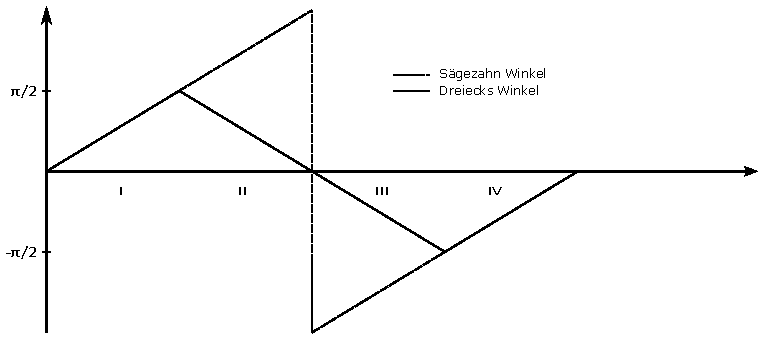
\includegraphics[width=0.53\textwidth]{Cordic_phi.pdf}
	\caption{berechneter Winkel \textit{phi} des Cordic Contrllers in Funktion der Zeit} 
	\label{img:Cordic_phi}
\end{figure}  


\paragraph{Mixer}\mbox{}\\

Die Implementation des Mixers ist dank der Entscheidung für die Rechteckform des analogen Oszillatorsignals sehr einfach. Über einen GPIO liest die Mixerkomponente das Signal des Antennenoszillators ein und verrechnet es mit dem generierten Sinus \textit{ref\_out}. Eine 1 des Rechtecks wird dabei als die Zahl 1 und eine 0 als die Zahl -1 interpretiert. Die Multiplikation zwischen der 1 und \textit{ref\_out} ist dabei nicht nötig und eine Multiplikation mit -1 erzielt der Mixer durch das Bilden des Zweierkomplement von \textit{ref\_out}.

\paragraph{Filter}\mbox{}\\
Im Projekt 5 war das Filter ein einzelnes CIC-Filter mit dem Decimationsfaktor 1000. Dies hatte zur Folge, dass viel Aliasing entstand. Um dieses zu verringern haben wir uns im Projekt 6 für den Aufbau aus Abbildung \ref{img:Filter_Pitch} entschieden. Die drei Filter CIC 1 bis CIC 3 sind Instanzen einer CIC-Filter Komponente. Diese Komponente ist unverändert geblieben seit Projekt 5. Die Parameter der drei Instanzen sind in Tabelle \ref{tab:cic_pitch} ersichtlich. Da es bei CIC-Filtern wie in Kapitel ... \todo{Referenz auf CIC-Filter Kapitel einfügen} beschrieben, um deren Nullstellen zu Aliasing kommt, sind diese Filter so eingestellt, dass sich die Oberwellen des Rechteck möglichst nicht in deren Nähe befinden. Bei CIC 1 wurde eine höhere Ordnung gewählt um am Anfang eine stärkere Dämpfung zu erzielen. Die Anzahl Ausgangsbits wurde nach Formel ... \todo{referenz auf Formel in Theorie einfügen} berechnet.\\
Zuletzt haben wir noch ein FIR-Filter implementiert um das Signal auf 48kHz unter abzutasten. Das Filter hat eine Passfrequenz von \SI{2}{kHz} und eine Stopfrequenz von \SI{24}{kHz} mit einer Dämpfung von 55dB. Wir entschieden uns die Koeffizienten mit dem filterDesigner Tool von Matlab zu berechnen und als \SI{27}{Bit} signed Zahlen in einer Lookup Table zu speichern. Wir wählten deshalb \SI{27}{Bit}, da im FPGA eine solche Multiplikation noch knapp in einen DSP Block integriert werden kann. \cite{Cyclone_V}
Weswegen der Ausgang Frequency Measurement nach dem zweiten CIC-Filter gewählt wurde ist im nächsten Abschnitt beschrieben.


\begin{figure}[h!]
	\centering
	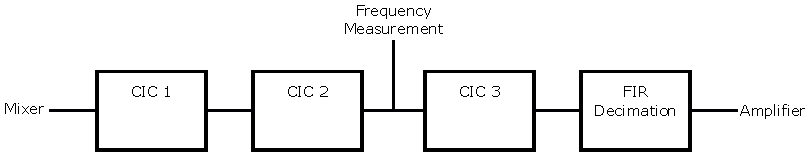
\includegraphics[width=1\textwidth]{Filter_pitch.pdf}
	\caption{Aufbau des Filters in der Komponente Pitch Generation} 
	\label{img:Filter_Pitch}
\end{figure}  

\begin{table}[H]
	\centering
	\caption{Parameter der drei CIC-Filter}
	\label{tab:cic_pitch}
	\begin{tabular}{l|l|l|l|l}
		\textbf{Komponente} & \textbf{Dezim.Fakt.} & \textbf{Ordnung} &  \textbf{Ausgangsfreq.} & \textbf{Ausgangsbits}\\
		\hline\hline
		CIC 1 & 5 & 2 & \SI{10.8}{MHz} & \SI{21}{Bits}  \\ \hline
		CIC 2 & 9 & 1  & \SI{12}{MHz} & \SI{25}{Bits}  \\ \hline
		CIC 3 & 5 & 1 & \SI{240}{kHz} & \SI{28}{Bits}  \\ \hline	
	\end{tabular}
\end{table}

\paragraph{Amplifier}\mbox{}\\

Die Komponente Amplifier ist dafür zuständig beim Signal \textit{filt\_out} den Gain der CIC-Filter zu kompensieren und anschliessend dieses mit der Dämpfung, welche die Volume Generation liefert, zu multiplizieren. In Abbildung \ref{img:Zero_Cross} ist eine Problematik aufgezeigt, welche auftritt, wenn man die Dämpfung zu beliebigen Zeiten wechselt. Links sieht man, was passiert, wenn die Dämpfung beim höchsten Wert der positiven Halbwelle ändert. Diese Sprünge im Signal treten dann als hörbares Knacksen auf. Um dies zu verhindern ist eine Erkennung von Nulldurchgängen implementiert, dass wie in der Abbildung rechts die Dämpfungen nur bei diesen Nullstellen geändert werden. Da der Codec ein Offsetbehaftetes Signal verlangt muss das MSB des Signal getoggelt werden um dies zu bewerkstelligen. Diese Komponente enthält zudem die Kommunikation mit dem Streaming Interface. \\
Die Dämpfung des Audiosignals könnte auch über den Codec gemacht werden. Weshalb dies nicht möglich ist, ist in Kapitel ... \todo{Referenz auf Software Audio} beschrieben. 
	
\begin{figure}[h!]
	\centering
	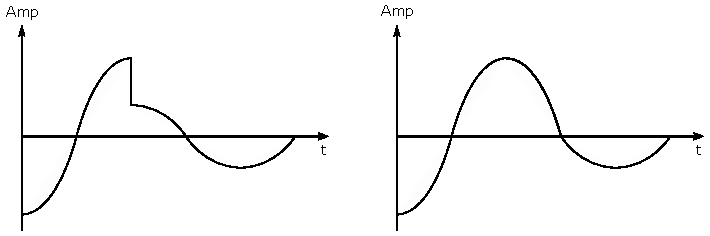
\includegraphics[width=1\textwidth]{Zero_Cross.pdf}
	\caption{Unterschied Dämpfungswechsel (links ohne und rechts mit Nullstellenerkennung)} 
	\label{img:Zero_Cross}
\end{figure}  


\paragraph{Frequenzmessung, Kalibration \& Glissandoeffekt}\mbox{}\\

Die Komponente Frequency Measurement hat mehrere Aufgaben und ist diejenige Komponente mit welcher über den Nios Prozessor die gesammte Pitch Generation gesteuert werden kann. Der Aufbau dieser Komponente ist in Abbildung \ref{freq_meas_pitch} aufgezeigt.\\
Zum einen wird hier die Frequenzmessung durchgeführt. Dies geschieht über die drei Komponenten FIR, Period Counter und Goldschmidt divider. FIR ist wie der Name sagt ein FIR Filter. Dieses ist nötig um das Signal aus dem Filter, welches noch Hochfrequente Signale enthält zu Filtern. Das Filter hat eine Grenzfrequenz von ... \todo{Grenzfrequenz und Dämpfung einfügen}. Das Filter wurde mit dem Tool filterDesigner in Matlab berechnet. Wir haben entschieden die Filterkoeffizienten als fixed-point signed Zahlen in einem Array mit \SI{18}{bit} länge abzuspeichern. Auf dieser Koeffizientenlänge kann Quartus die DSP-Blöcke so nutzen, dass nach der Multiplikation des Signals mit den Koeffizienten die Resultate gleich in den Blöcken addiert wird. Dies ermöglicht längereMultiplikationsketten. \todo{Nochmal über DSP blöcke nachlesen und referenzieren} \\
Anschliessend wird das Signal \textit{fir\_out} im \textit{Period Counter} ausgemessen. Diese zählt von Nulldurchgang zu Nulldurchgang einen Zähler hoch. Bei einem Nulldurchgang wird der Wert dieses Zählers am Signal \textit{per\_cnt} ausgegeben. Der Zählerwert entspricht der Anzahl Abtastwerte des Signals in einer Signalperiode. \\
Das Signal hat eine Abtastfrequenz von \SI{1.2}{MHz}. Dividiert man diese Abtastfrequenz durch die zuvor gezählte Anzahl Abtastperioden erhält man die Frequenz des Signals.\\ Um diese Division zu berechnen haben wir uns entschieden den Goldschmidt Algorithmus aus Kapitel ... \todo{referenz auf theorie goldschmidt einfügen} einzusetzen. Dieser hat den Vorteil, dass er auch Nachkommastellen berechnen kann um die nötige Genauigkeit bei den Tiefen Frequenzen zu erreichen wie in Kapitel ... \todo{Referenz auf Musikkapitel einfügen} beschrieben. Dass die Berechnungsdauer des Algorithmus nicht für alle Zahlen gleich ist, ist nicht Problematisch, da diese Zeiten im Nanosekundenbereich liegen und nicht hörbar sind.

\begin{figure}[h!]
	\centering
	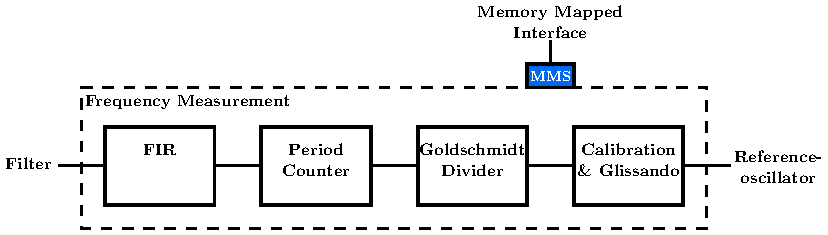
\includegraphics[width=1\textwidth]{freq_meas_pitch.pdf}
	\caption{Aufbau der Frequenzmessung, Kalibration und Glissandoeffekt in der Komponente Pitch Generation} 
	\label{img:freq_meas_pitch}
\end{figure}  
\todo{Bild überarbeiten und namen an Signalen anbringen wie in Text}

Die gemessene Frequenz wird anschliessend in der Komponente \textit{Calibration \& Glissando} benötigt. Diese ist dafür zuständig einerseits die Tonhöhe zu kalibrieren und andererseits den Glissando-Effekt zu steuern. Um die Frequenz des Referenzoszillator zu steuern wird die Differenz welche den Glissandoeffekt hervorruft und die Änderung welche während der Kalibration berechnet wurde addiert und dem Referenzoszillator als Frequenzdifferenz übergeben. Die Steuerung dieser Funktionen ist als State-Machine aufgebaut wie in Abbildung \ref{img:state_event_Cal_Glis} zu sehen ist. Es folgt eine Erklärung, was in den einzelnen Zuständen geschieht:

\textbf{Idle}:
Sind beide Funktionen deaktiviert, wird das die Frequenznderung des  zum Referenzoszillator auf 0Hz gesetzt.

\begin{figure}[h!]
	\centering
	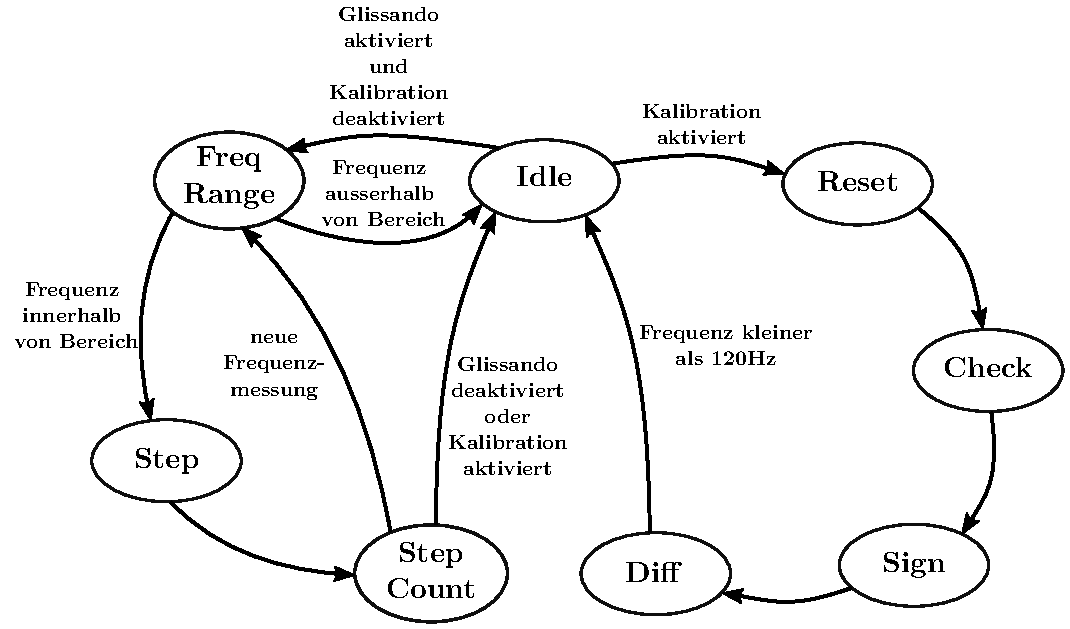
\includegraphics[width=1\textwidth]{state_machine_Cal_Glis.pdf}
	\caption{State Event Diagramm der Kalibration \& Glissando Komponente} 
	\label{img:state_event_Cal_Glis}
\end{figure} 